\documentclass[frenchb]{article}
\usepackage[T1]{fontenc}
\usepackage[utf8]{inputenc}
\usepackage[francais]{babel}
\usepackage{fancyhdr}
\usepackage{float}
\usepackage{lastpage}
\usepackage{fancyvrb} 
\usepackage{graphicx}
\usepackage{hyperref}
\usepackage{soul}
\usepackage{listings}
\usepackage{xcolor}

\definecolor{mygreen}{rgb}{0,0.6,0}
\definecolor{mygray}{rgb}{0.3,0.3,0.3}
\definecolor{mymauve}{rgb}{0.58,0,0.82}

\lstset{ %
  backgroundcolor=\color{white},   % cbackground color \usepackage{xcolor}
  basicstyle=\footnotesize,        % font size
  breakatwhitespace=false,         % autobreak only at whitespace
  breaklines=true,                 % sets automatic line breaking
  captionpos=b,                    % sets the caption-position to bottom
  commentstyle=\color{mygreen},    % comment style
  deletekeywords={...},            % delete keywords from the given language
  escapeinside={\%*}{*)},          % if you want to add LaTeX within your code
  extendedchars=true,              % lets you use non-ASCII characters; no UTF8
  frame=single,                    % adds a frame around the code
  keepspaces=true,                 % keeps spaces, to indent : columns=flexible
  keywordstyle=\color{blue},       % keyword style
  language=Octave,                 % the language of the code
  morekeywords={*,...},            % if you want to add more keywords to the set
  numbers=left,                    % where to put line number (none, left, right)
  numbersep=5pt,                   % how far the line-numbers are from the code
  numberstyle=\footnotesize\color{mygray}, % line number style
  rulecolor=\color{white},         % black for rules
  showspaces=false,                % show spaces, overrides 'showstringspaces'
  showstringspaces=false,          % underline spaces within strings only
  showtabs=false,                  % show tabs 
  stepnumber=1,                    % the step between two line-numbers.
    stringstyle=\color{mymauve},     % string literal style
  tabsize=2,                       % sets default tabsize to 2 spaces
  title=\lstname                   % filename \lstinputlisting; try caption
}

\lstdefinestyle{customc}{
  belowcaptionskip=1\baselineskip,
  breaklines=true,
  frame=L,
  xleftmargin=\parindent,
  language=C,
  showstringspaces=false,
  basicstyle=\normalsize\ttfamily,
  keywordstyle=\bfseries \color{green!40!black},
  commentstyle=\itshape \color{purple!40!black}, %itshape
  identifierstyle=\color{blue},
  stringstyle=\color{orange},
}
\lstset{escapechar=@,style=customc}


\pagestyle{fancy}
\lhead{Projet Olimex}
\cfoot{M.BRULATOUT - A.DUFORAT - L.L\'EV\^EQUE - K.MALLOUKY - N.SARLIN}
\rfoot{\thepage}
\renewcommand{\footrulewidth}{0.5pt}
\begin{document}
\topmargin        = 0.mm
\headheight       = 12.1638pt
\evensidemargin   = 10.mm
%\oddsidemargin    = 10.mm
%\textheight       = 215.mm
%\textwidth        = 145.mm
\begin{titlepage}
  \begin{center}
    \textsc{\LARGE Rapport du projet PR311 : Olimex}\\[0.5cm]
    \textsc{\Large Mathias BRULATOUT\\ Arnaud DUFORAT\\ Louis L\'EV\^EQUE\\ Kamal MALLOUKY\\ Nicolas SARLIN}\\[1.5cm]
    \textsc{\Large \today }\\[1.5cm]
    \begin{figure}[h!]
      \center
      \includegraphics[width=8cm]{enseirb.png}
    \end{figure}
    \vspace{1cm}
    \textsc{\Large Responsable Pédagogique : Aymeric Vincent}
  \end{center}  
\end{titlepage}
%\tableofcontents
\section*{Introduction}
Dans le cadre du projet PR311 Développement système, il a été choisi de développer sur un Olimex OLinuXino A20. Pour en savoir plus sur la programmation bas niveau, nous avons décidé d'implémenter un pseudo-OS,  plutôt que d'utiliser une plateforme UNIX pour développer quelque chose ayant un intérêt pédagogique bien plus limité.

Ce rapport explique les démarches que nous avons adoptées pour mener à bien ce projet, les choix que nous avons fait et les raisons pour lesquelles nous les avons faits.

Tout d'abord, l'A20 sera presenté, afin d'enchaîner sur le travail et les choix effectués.
\clearpage
\section{Présentation de la plateforme}

\subsection{OLinuXino A20}
L'Olinuxino est un nano-ordinateur, composé d'une carte mère distribuée en matériel libre basé sur un système sur puce. Il s'agit d'un système embarqué sur une seule puce ARM. Cette unique puce intègre un mircoprocesseur dual core, de la mémoire vive, une mémoire flash, un connecteur micro SD et différents connecteurs tels que des ports USB etc. La puce intégre aussi 3 connecteurs GPIO regroupant un ensemble de 160 pins controlables, et une connection série sur laquelle nos travaux ont été focalisés.

L'A20 était doté dès le départ d'un système Android stocké sur la mémoire flash de l'équipement. Cependant, faire un projet de développement système sur un système Android n'était pas d'un grand intérêt, ni même installer un système UNIX sur une carte SD et le faire tourner sur l'Olinuxino pour faire du développement. Notre curiosité nous a poussé plus loin et nous avions décidé de developper un pseudo OS en C qui permettra de communiquer sur le port série via l'utilisation d'un UART et de manipuler les GPIO de la carte.

Plutôt que de développer un OS baremetal et de passer plus de temps à faire fonctionner les divers périphériques plutôt que de les utiliser, nous avons choisi d'utiliser Uboot, chargeur de démarrage nous permettant d'envoyer un binaire pouvant utiliser les différents périphériques sur la carte et de l'exécuter.
 
\subsection{U-boot}

Uboot (Universal Bootloader) est un chargeur de démarrage écrit en C permettant d'amorcer un Système d'exploitation sur un équipement particulier et fonctionne sur plusieurs architectures. Il est en général exécuté lors de la mise sous tension de l'équipement dans le but d'initialiser les périphériques. Uboot démarre à partir d'une ROM, et peut utiliser un cache de données ou une puce du processeur comme mémoire vive.

Après avoir récupéré et compilé les sources les plus récentes de U-boot via le git approprié à notre plateforme, il nous a fallu répeter de nombreuses fois la même manipulation avant de se rendre compte que la version la plus récente de U-boot ne marchait pas. Il nous a donc fallu revenir à une version antérieure.
Pour mettre U-boot sur une carte Micro SD, deux partitions ont été crées : la première formatée en vfat qui est le format attendu par le bootloader et la deuxième en ext2 si on veut mettre des binaires dessus :

\begin{itemize}
  \item \textsf{mkfs.vfat /dev/sdb1}
  \item \textsf{mkfs.ext2 /dev/sdb2}
 \end{itemize}

Il ne restait plus qu'à écrire grâce à un dd sur /dev/sdb, U-boot avec un SPL (Secondary Program Loader), qui se appelé par le bootloader et qui chargera U-boot :

\begin{verbatim}
dd if=u-boot-sunxi/u-boot-sunxi-with-spl.bin of=/dev/sdb bs=1024 seek=8
\end{verbatim}

Après compilation du code sans l'inclusion de la moindre bibliothèque externe et avec un grand nombre d'options via la commande \textsf{arm-linux-gnueabihf-gcc}, il suffit d'envoyer le binaire généré sur l'Olimex relié par un port USB série en utilisant la commande ckermit du coté client et loadb du coté Olimex.
Après l'envoi du binaire de l'OS sur une adresse bien spécifique au niveau de l'Olimex, il ne reste plus qu'à se positionner sur l'adresse en question et exécuter le binaire.

\section{UART}
Une fois que nous avons réussi à compiler et exécuter notre propre programme sur la carte, il a fallu développer ce qui allait être la base de l'interface de notre système : la communication série.
Pour cela il nous faut utiliser un UART (Universal Asynchronous Receiver Transmitter), composant dédié à ce type de communication.
Puisque l'UART0 est doté d'un brochage séparé et que c'est celui utilisé par la console U-Boot, nous avons décidé de l'utiliser nous aussi.
En cherchant dans le manuel d'utilisation du processeur A20, nous avons rapidement trouvé les informations nécessaires à l'utilisation du premier UART intégré :
\begin{itemize}
\item L'adresse de base de l'UART à partir de laquelle sont placés tous ses registres.
\item La liste des registres de contrôle et de données de l'UART.
\end{itemize}
Après avoir réussi à envoyer un octet en assignant une valeur au registre DAT, nous avons écrit trois fonctions permettant d'initialiser la communication, d'envoyer et de recevoir un caractère.

Le fichier \textsf{uart.h} contient les différentes adresses de l'UART nécessairesà l'usage que l'on en fait, à savoir la simulation d'un terminal (lecture/écriture de caractères).

\begin{lstlisting}
 /*UART0 address*/
#define UART0 0x01C28000
/*UART0's FIFO Control Register Offset*/
#define FCR (1 << 1)
/*UART0's Line Status Register offset*/
#define LSR 5
/*Data Ready Bit : First bit in LSR*/
#define DR 0x1

/*TX Holding Register Empty Bit : Sixth bit in LSR*/
#define THRE (1 << 5)
\end{lstlisting}
\vspace*{-0.8cm}

Le registre FCR (FIFO Control Register) nous permet de désactiver la gestion de file, pour nous faciliter la tâche.
L'idée est ensuite de manipuler le registre LSR (Line Status Register) et son bit DR (Data Ready) pour récupérer un caractère lorsque ce bit est égal à 1. Cela nous permet de simuler une fonction \textsf{getc}.

 Le bit THRE (Tx Holding Register Empty) du même registre est à 1 lorsque le mode FIFO est désactivé et lorsqu'un caractère est prêt à être reçu. Il ne reste plus qu'à écrire le caractère reçu pour simuler un \textsf{putc}.

En se basant sur la fonction d'envoi, nous avons pour plus de commodité créer une fonction destinée à envoyer une chaîne de caractères.

L'étape suivante à été naturellement de réaliser l'interface console à proprement dite. Une fonction est chargée d'afficher le prompt, une autre qui doit être appelée à intervalles réguliers, s'occupe de recevoir les frappes clavier et de renvoyer les caractères reçus afin de fournir un retour à l'utilisateur. Cette même fonction stocke les caractères dans un buffer, et appelle la fonction d'exécution de commande si l'utilisateur a pressé la touche Entrée.

%\lstinputlisting[caption=Scheduler, style=customc]{../uart.c}
\section{GPIO}
Les GPIO (General Purpose Input Output) sont des modules d'entrées sorties permettant d'interfacer le SoC à toutes sortes d'éléments, notamment des LEDs ou des boutons.
L'OLinuXino dispose de 3 connecteurs GPIO. Nous avons choisi d'utiliser le GPIO0. Du point de vue du contrôleur, 10 ports peuvent être utilisés pour remplir diverses fonctions telles que des bus de communications SPI, CAN, TWI et UART. Il est également possible d'utiliser certains ports comme source d'interruption. Dans ce projet on considère uniquement leur fonction GPIO.
Chaque port dispose de jusqu'à 4 registres de configuration permettant de choisir pour chaque broche du port si elle doit être utilisé comme entrée, sortie ou pour une fonction avancée.
La configuration d'une broche se fait sur 3 bits mais ces configurations sont alignées sur 4 bits dans le registre qui concerne donc uniquement 8 broches. La combinaison \so{\textsf{001}} correspond à une sortie alors que \so{\textsf{000}} correspond à une entrée.
Une fois que les broches sont configurées, on peut lire ou écrire le registre DAT du port où chaque bit correspond à une broche.
La LED intégrée à la carte est elle même raccordée à un GPIO ce qui permet de la contrôler de manière logicielle.
Pour les contrôler, nous avons créé deux commandes. La première est led, qui sans paramètre change l'état de la LED1. Elle peut aussi accepter un entier (0 ou 1) pour allumer ou éteindre la LED. En cas de mauvaise utilisation, nous affichons un usage. La deuxième est gpio, qui sans paramètre active la pin 9 du GPIO-2. Elle active la pin voulue en lui passant en paramètre le numéro de cette pin.
\section{Memory Management}

\subsection{Detection de la mémoire}
Notre premier objectif était de pouvoir détecter la mémoire de manière automatique, indépendante du matériel. Par exemple, on voudrait pouvoir utiliser notre gestionnaire de mémoire quelle que soit la quantité de RAM disponnible.  Si sur architecture x86 il est possible d'interroger très simplement le BIOS pour obtenir les informations voulues, ça n'est pas le cas sur ARM. Des recherches nous orientent vers une méthode de \textit{manual probing}. Le principe est de tester sur l'ensemble de l'espace adressable, à intervalle régulier (ici tous les Mio), si une valeur peut-être écrite puis lue sans erreur. Pour éviter d'effacer des données importantes en mémoire (exemple : le code de notre fonction), on sauvegarde dans une variable la valeur qui était présente à cette adresse avant notre test. On cherche ensuite à détecter la plus longue séquence possible sans erreurs, et on considère qu'il s'agit de la RAM. Cette méthode n'est bien sûr pas parfaite. En effet, on ne prend pas en compte des effets non voulus, tels que l'écriture dans des caches, ou une \textit{persistance} des bus qui ferait qu'une valeur écrite puis lue directement après serait en fait un résidu présent dans le bus. Il faut aussi, évidemment, s'assurer que le compilateur ne fera pas d'optimisation. \\ \\
En testant cette méthode, puis en comparant les résultats avec des valeurs connues (1G de RAM, débutant à l'adresse 0x40000000), on tombe sur des résultats \textit{presque cohérents}. La zone détectée est beaucoup plus grande que la zone mémoire réelle. En comparant avec la documentation du processeur, on comprend qu'on écrit à certaines adresses en dehors de celles dédiées à la mémoire. De plus, notre test détecte que tout l'espace d'adressage dédié à la mémoire est utilisé, comme si nous avions en réalité 4G de RAM. Nous avons effectué une petite expérience supplémentaire pour comprendre ce phénomène:\\
Nous écrivons à des adresses 0x400000XX, puis lisons aux adresses 0x800000XX (soit aux valeurs \textit{adresse+1G}). A chaque fois, la valeur lue est égale à celle écrite. Cela s'explique par le fait qu'en l'absence de mémoire, l'adressage est répété, et plusieurs adresses vont pointer sur le meme espace physique.\\ \\
La détection de mémoire automatique n'est donc pas efficace dans notre cas, ou du moins n'avons nous pas eu le temps d'approfondir suffisemment pour obtenir quelque chose d'exploitable. Pour la suite du développement, nous utilisons donc des valeurs trouvées dans la documentation ou detectées par expérimentation pour placer notre tas. Par exemple, il est possible d'afficher le contenu des registres en insérant du code assembleur dans notre C :
\begin{lstlisting}

    unsigned int spReg, lrReg, pcReg;

    asm volatile ("mov %0, sp" :
                "=r" (spReg));
    
    asm volatile ("mov %0, lr" :
                "=r" (lrReg));

    asm volatile ("mov %0, pc" :
                "=r" (pcReg));
\end{lstlisting}
La fonction \textsf{asm volatile ("instruction \%0, \%1":"=r" (output):"r" (input))} permet d'indiquer à GCC que l'on souhaite placer l'instruction assembleur \textit{instruction \%0, \%1} dans notre code, et que l'on souhaite utiliser que l'entrée soit lue dans la variable C input, et la sortie écrite dans la variable output. Ainsi, on repère l'emplacement mémoire où se situe le code gràce à pc et lr, et celui où se situe la stack avec pc. On voit donc qu'au lancement le code est placé au début de la RAM, et la stack à la fin. Nous plaçons donc notre tas \textit{au milieu} (Notre système étant monoprocess, nous n'avons qu'un seul tas).

\subsection{Gestionnaire de mémoire}
Une fois en possession d'une zone mémoire où nous pouvons écrire sans craindre d'affecter le reste du fonctionnement de la machine (\textit{le milieu}), reste à définir des fonctions permettant au reste de notre système d'y reserver et libérer de la mémoire. Nous appellerons arbitrairement ces fonctions \textit{malloc} et \textit{free}.\\
Pour implémenter ces fonctions, nous devons faire un choix de représentation de notre mémoire. Nous choisissons de conserver un petit espace supplémentaire juste avant l'adresse retournée par malloc:\\
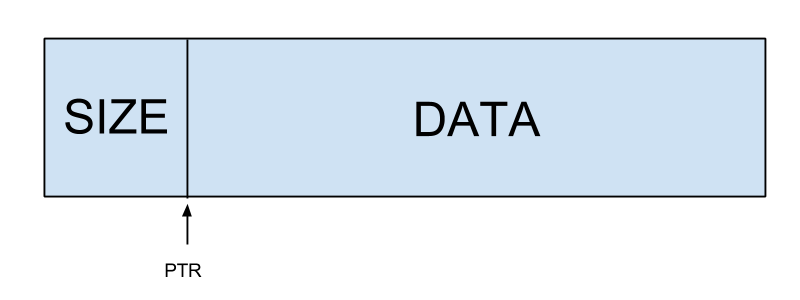
\includegraphics[width=8cm]{memblock.png}\\
Ainsi, free pourra savoir quelle quantité de mémoire libérer uniquement à partir du pointeur qui lui est passé. On maintient un pointeur vers le dernier espace alloué, \textsf{firstfree}. Malloc distingue deux cas avant d'agir : Soit la mémoire déjà allouée est continue, soit des blocs libres se trouvent en plein milieu. Dans le premier cas, il suffit simplement de recupérer la valeur de \textsf{firstfree} dans une variable (\textsf{addr}),d'ecrire la taille allouée à l'adresse \textsf{addr-sizeof(int)}, puis d'incrémenter \textsf{firstfree} de \textsf{taille + sizeof(int)}. Le second cas va dépendre du comportement que l'on choisit pour free.\\
Pour free, nous maintenons une liste doublement chainée des blocs libres qui sont suivis d'au moins un bloc alloué. Si on essaie de libérer le dernier bloc du tas, free va simplement mettre à jour la valeur de \textsf{firstfree}. Dans le cas contraire, on rajoute simplement le bloc à la liste (par son adresse), de manière à ce que les blocs de la liste soient organisés par adresse croissante. Ainsi, lorsqu'un malloc futur sera fait, malloc va parcourir cette liste à la recherche d'un bloc libre dont la taille serait supérieure à la la taille que l'on souhaite allouer. \\\\
Nos mallocs et free fonctionnent et permettent d'allouer des blocs de mémoire de taille quelconque, de les libérer dans n'importe quel ordre puis de réallouer dans les emplacements libres. Dans un avenir proche, nous avions prévu d'améliorer la libération en fusionnant deux blocs libre continus dans la liste chainée (D'où l'intéret de la liste doublement chainée). Notre fonction malloc retourne \textsf{NULL} quand la taille de notre tas risque d'empiéter sur les autres zones mémoire. 

\clearpage

\section*{Conclusion}

\noindent Ce projet a été l'occasion de programmer à un niveau plus bas que nous ne l'avons jamais fait. Nous avons pu utiliser le C sans bibliothèque, et utiliser les UARTs et GPIO qui nous étaient inconnus avant ce projet.
De nombreux problèmes ont été rencontrés tout au long du projet, dont la regression constatée sur la dernière version de U-boot et notre manque de pratique du C bas niveau. 
Nous avons aussi réussi à implémenter un module de gestion mémoire via malloc et free.
Cependant, il y a encore de nombreuses étapes à parcourir pour obtenir un vrai système d'exploitation, notamment la gestion de la MMC, l'implémentation d'un système de fichiers ou l'exécution de programmes. Nous n'avons jamais perdu de vue ces fonctionnalités ce qui nous a aidé à écrire un code modulaire et maléable.

\end{document}
